\documentclass{article}
\usepackage{import}
\usepackage{amsmath}
\usepackage{tabularray}
\usepackage{float}


\import{lib/latex/}{wgmlgz}
\patchcmd{\thebibliography}{\section*}{\section}{}{}

\begin{document}
\itmo[
      variant=13,
      labn=4,
      discipline=Вычислительная математика,
      group=P3212,
      student=Соколов Анатолий Владимирович,
      teacher=Наумова Надежда Александровна 
]
\lstset{language=rust}
\newgeometry{
  a4paper,
  top=20mm,
  right=10mm,
  bottom=20mm,
  left=30mm
}
\tableofcontents
\section{Задание}
      \subsection{Вычислительная реализация задачи}

      Вычислительная часть лабораторной работы должна быть представлена только в отчете.

            \textbf{Задание:}
            \begin{enumerate}
            \item Сформировать таблицу табулирования заданной функции на указанном интервале (см. табл. 4.1).
            \item Построить линейное и квадратичное приближения по 11 точкам заданного интервала.
            \item Найти среднеквадратические отклонения для каждой аппроксимирующей функции. Ответы дать с тремя знаками после запятой.
            \item Выбрать наилучшее приближение.
            \item Построить графики заданной функции, а также полученные линейное и квадратичное приближения.
            \item Привести в отчете подробные вычисления.
            \end{enumerate}

      \subsection{Программная реализация задачи}

            Для исследования использовать:
            \begin{itemize}
            \item линейную функцию,
                  \item полиномиальную функцию 2-й степени,
                  \item полиномиальную функцию 3-й степени,
                  \item экспоненциальную функцию,
                  \item логарифмическую функцию,
                  \item степенную функцию.
            \end{itemize}

            \textbf{Методика проведения исследования:}
            \begin{enumerate}
                  \item Вычислить меру отклонения для всех исследуемых функций.
                  \item Уточнить значения коэффициентов эмпирических функций, решая для этого системы линейных уравнений.
                  \item Сформировать массивы предполагаемых эмпирических зависимостей.
                  \item Определить среднеквадратичное отклонение для каждой аппроксимирующей функции. Выбрать наименьшее значение и, следовательно, наилучшее приближение.
                  \item Построить графики полученных эмпирических функций.
            \end{enumerate}

            \textbf{Задание:}
            \begin{enumerate}
                  \item Предусмотреть ввод исходных данных из файла/консоли (таблица должна содержать от 8 до 12 точек).
                  \item Реализовать метод наименьших квадратов, исследуя все указанные функции.
                  \item Предусмотреть вывод результатов в файл/консоль: коэффициенты аппроксимирующих функций, среднеквадратичное отклонение, массивы значений.
                  \item Для линейной зависимости вычислить коэффициент корреляции Пирсона.
                  \item Программа должна отображать наилучшую аппроксимирующую функцию.
                  \item Организовать вывод графиков функций, графики должны полностью отображать весь исследуемый интервал (с запасом).
                  \item Программа должна быть протестирована при различных наборах данных, в том числе и некорректных.
            \end{enumerate}

\subsection{Вариант}

Варианты задания для вычислительной реализации задачи: 
 $$y=\frac{31x}{x^4+13}, x\in[0;4], h=0.4$$

\subsection{Цель работы}
      Найти приближенное значение определенного интеграла с требуемой точностью различными численными методами.

\section{Выполнение}

      
      \subsection{Табулирование функции}

            Первым делом сформируем таблицу значений функции \(y=\frac{31x}{x^4+13}\) на интервале \([0;4]\) с шагом \(h=0.4\). То есть, мы будем вычислять значение функции в точках \(x=0, 0.4, 0.8, \ldots, 4\).

            Выполним эти вычисления:

            Мы получили таблицу табулирования функции \(y=\frac{31x}{x^4+13}\) на интервале от 0 до 4 с шагом 0.4. Вот её значения:

            \[
            \begin{array}{|c|c|}
            \hline
            x & y \\
            \hline
            0.0 & 0.000 \\
            0.4 & 0.952 \\
            0.8 & 1.849 \\
            1.2 & 2.468 \\
            1.6 & 2.537 \\
            2.0 & 2.138 \\
            2.4 & 1.611 \\
            2.8 & 1.166 \\
            3.2 & 0.842 \\
            3.6 & 0.617 \\
            4.0 & 0.461 \\
            \hline
            \end{array}
            \]

      \subsection{Линейное и квадратичное приближения}

            Теперь найдем линейное (первой степени) и квадратичное (второй степени) приближения для этой функции, используя метод наименьших квадратов. Приближения будут иметь вид \(y = ax + b\) для линейного и \(y = ax^2 + bx + c\) для квадратичного.

      \subsubsection{Линейное приближение}

            Для линейного приближения мы используем формулу метода наименьших квадратов:

            \[
            n a + \left(\sum x_i\right) b = \sum y_i \\
            \left(\sum x_i\right) a + \left(\sum x_i^2\right) b = \sum x_i y_i
            \]

            Подставляем реальные значения:

            \[
            \begin{aligned}
            11a + (22)b &= 15.34 \\
            22a + 60.8b &= 45.96
            \end{aligned}
            \]

            Решая систему, находим \(a\) и \(b\).
            \(a = 1.585\), \(b = -0.127\)

      \subsubsection{Квадратичное приближение}

            Аналогично, для квадратичного приближения найдем коэффициенты \(a\), \(b\), и \(c\), решив соответствующую систему уравнений.

            Приступим к вычислениям коэффициентов:


            \[
            \begin{aligned}
            n a + \left(\sum x_i\right) b + \left(\sum x_i^2\right) c &= \sum y_i \\
            \left(\sum x_i\right) a + \left(\sum x_i^2\right) b + \left(\sum x_i^3\right) c &= \sum x_i y_i \\
            \left(\sum x_i^2\right) a + \left(\sum x_i^3\right) b + \left(\sum x_i^4\right) c &= \sum x_i^2 y_i
            \end{aligned}
            \]
            
            Сначала вычислим необходимые суммы:
            
            - \(S_x = \sum x_i\)
            - \(S_{x^2} = \sum x_i^2\)
            - \(S_{x^3} = \sum x_i^3\)
            - \(S_{x^4} = \sum x_i^4\)
            - \(S_y = \sum y_i\)
            - \(S_{xy} = \sum x_i y_i\)
            - \(S_{x^2y} = \sum x_i^2 y_i\)

            
            Все необходимые суммы:
            
            - \(S_x = 22\)
            - \(S_{x^2} = 61.6\)
            - \(S_{x^3} = 193.6\)
            - \(S_{x^4} = 648.5248\)
            - \(S_y = 14.640\)
            - \(S_{xy} = 27.044\)
            - \(S_{x^2y} = 62.341\)
            
            Мы можем подставить их в систему уравнений для квадратичного приближения:
            
            \[
            \begin{aligned}
            11a + 22b + 61.6c &= 14.640 \\
            22a + 61.6b + 193.6c &= 27.044 \\
            61.6a + 193.6b + 648.5248c &= 62.341
            \end{aligned}
            \]
            
            Эту систему уравнений можно решить, чтобы найти коэффициенты \(a\), \(b\), и \(c\). Решение системы дает:
            
            - \(a \approx 0.416\)
            - \(b \approx 1.822\)
            - \(c \approx -0.487\)
            \\
            \textbf{Результаты}
            
            Коэффициенты линейного приближения получились как \(y = 1.585x - 0.127\), а коэффициенты квадратичного приближения как \(y = 0.416x^2 + 1.822x - 0.487\).

      \subsubsection{Нахождение СКО}

            Для линейного приближения у нас есть формула \(\hat{y}_i = 1.585x_i - 0.127\). СКО вычисляется как:

            \[
            \text{СКО} = \sqrt{\frac{1}{n} \sum (y_i - \hat{y}_i)^2}
            \]

            Для квадратичного приближения формула выглядит как \(\hat{y}_i = 0.416x_i^2 + 1.822x_i - 0.487\). Процесс аналогичен линейному приближению, но с использованием этой формулы.
            
            Разность для первой точки:

            \[
            y_1 - \hat{y}_1 = 0 - (-0.487) = 0.487
            \]

            Подставим значения для первой точки:

            \[
            \hat{y}_1 = 0.416 \cdot 0^2 + 1.822 \cdot 0 - 0.487 = -0.487
            \]

            Проведя аналогичные расчеты для всех точек, суммируем полученные квадраты разностей и делим на общее количество точек \(n = 11\), после чего извлекаем квадратный корень из результата.
            \begin{table}[htbp]
                  \centering
                  \label{tab:my-table}
                  \begin{tabular}{@{}cccccc@{}}
                        \(x\) & Линейное откл. & Квадрат. откл. & Квадрат лин. откл. & Квадрат квадр. откл. \\ 
                        0.0   & -1.585         & -0.416          & 2.512               & 0.173                 \\
                        0.4   & -0.582         & -0.115          & 0.339               & 0.013                 \\
                        0.8   & 0.366          & 0.288           & 0.134               & 0.083                 \\
                        1.2   & 1.035          & 0.568           & 1.072               & 0.322                 \\
                        1.6   & 1.155          & 0.453           & 1.334               & 0.206                 \\
                        2.0   & 0.807          & 0.028           & 0.651               & 0.001                 \\
                        2.4   & 0.331          & -0.370          & 0.110               & 0.137                 \\
                        2.8   & -0.064         & -0.531          & 0.004               & 0.282                 \\
                        3.2   & -0.337         & -0.415          & 0.113               & 0.172                 \\
                        3.6   & -0.511         & -0.043          & 0.261               & 0.002                 \\
                        4.0   & -0.616         & 0.553           & 0.379               & 0.306                 \\
                  \end{tabular}
                  \caption{Отклонения}
              \end{table}

      
      \subsubsection{Расчет и Сравнение СКО}

            После выполнения этих шагов для всех точек интервала, мы получаем СКО для линейного и квадратичного приближений:
            \[
            \text{СКО} = \sqrt{\frac{1}{n} \sum (y_i - \hat{y}_i)^2}
            \]
            \[
            \text{СКО (лин)} = \sqrt{\frac{1}{11} 2.63}
            \]
            \[
            \text{СКО (кв)} = \sqrt{\frac{1}{11}1.303 }
            \]

            СКО (линейное приближение) $\approx 0.793$ 
            
            СКО (квадратичное приближение) $\approx 0.393$

            Эти расчеты показывают, что квадратичное приближение обеспечивает меньшее среднеквадратическое отклонение, что говорит о его более высокой точности по сравнению с линейным приближением для данной функции и заданного интервала.

            Среднеквадратическое отклонение для линейного приближения составляет $0.793$, а для квадратичного приближения — $0.393$. Это означает, что квадратичное приближение лучше аппроксимирует данную функцию на выбранном интервале, так как имеет меньшее среднеквадратическое отклонение.

      \subsection{Выбор наилучшего приближения}

            На основе среднеквадратических отклонений, наилучшим приближением является квадратичное, так как его СКО меньше.

      \subsection{Построение графиков}

            Теперь построим графики исходной функции и аппроксимаций.  
            \\
            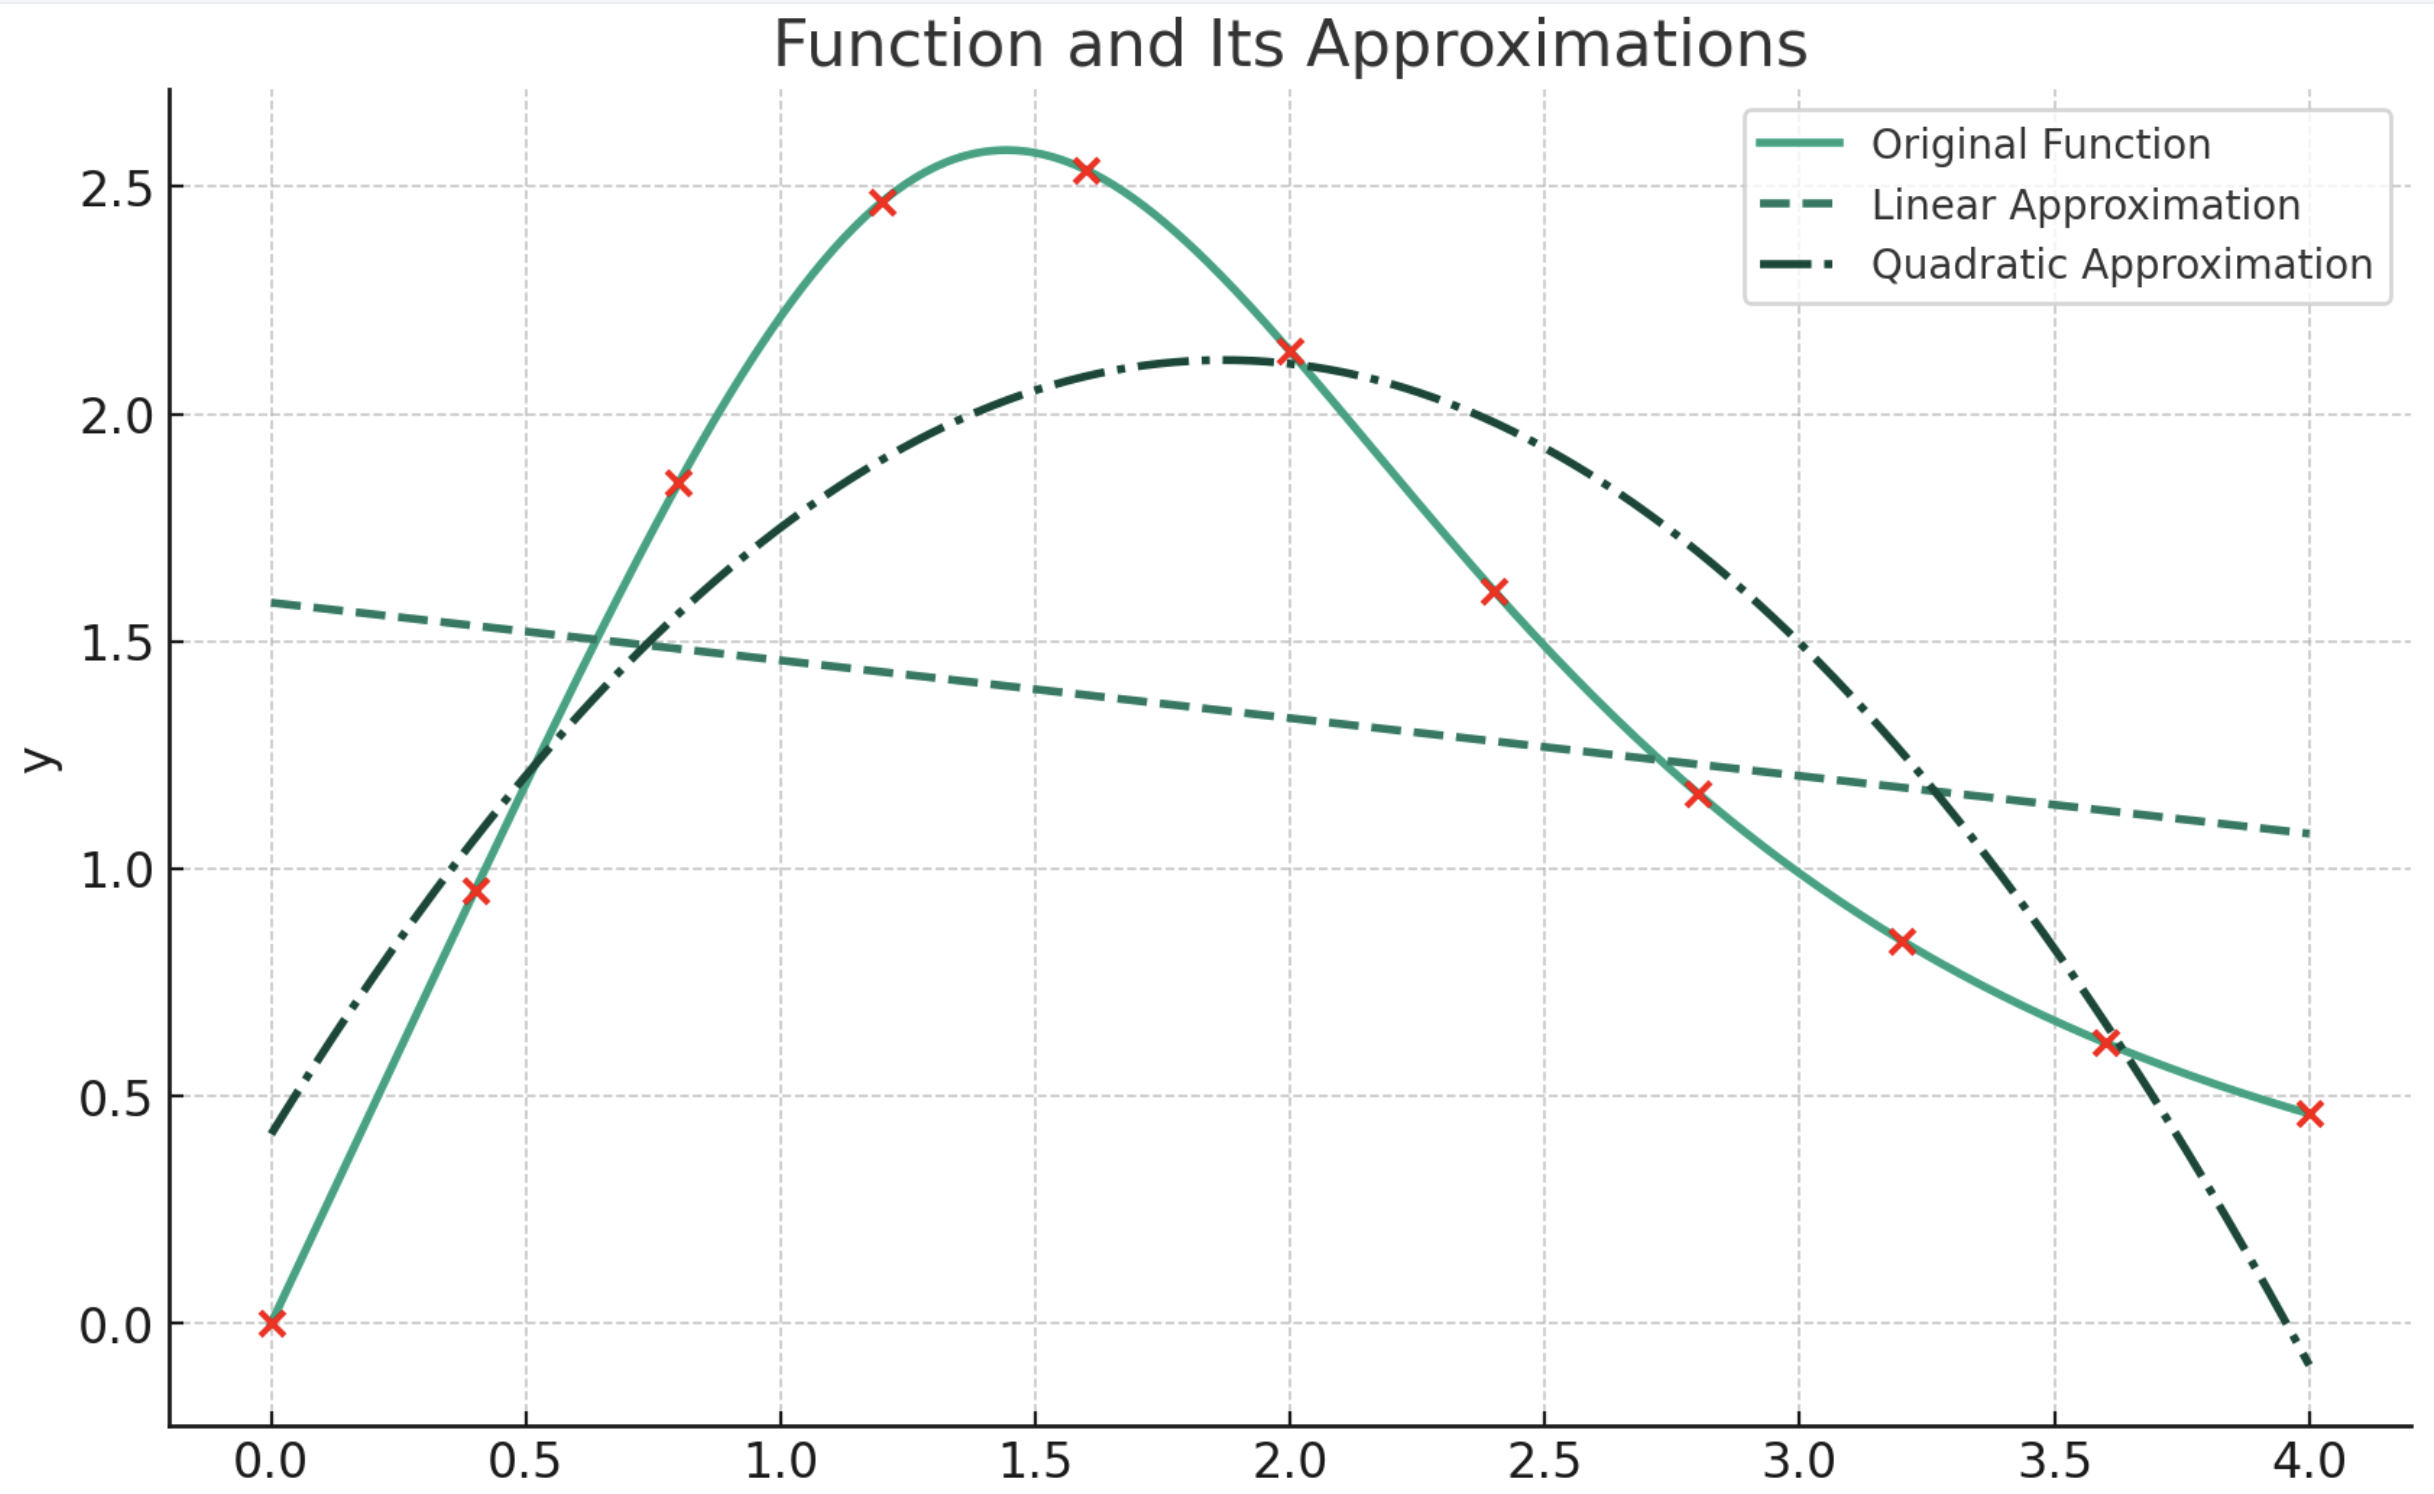
\includegraphics[scale=0.4]{hand_approx.png} 
      
      \subsection{Вывод}

            На основе среднеквадратического отклонения мы определили, что квадратичное приближение лучше подходит для аппроксимации данной функции, поскольку оно дает меньшее значение СКО.

      \subsection{Блок-схема реализованного алгоритма}
             
\includegraphics[scale=0.2]{best_function.png}
             \\
             
\includegraphics[scale=0.2]{exp_approx.png}
             \\
             
\includegraphics[scale=0.2]{lin_calc.png}
             \\
             
\includegraphics[scale=0.2]{log_approx.png}
             \\
             
\includegraphics[scale=0.2]{polynom_approx.png}
             \\
             
\includegraphics[scale=0.2]{power_approx.png}
             
      \subsection{Ссылка на GitHub c основной реализацией}
            \href{https://github.com/isofinly/compmath}{Github}

      \subsection{Примеры и результаты работы программы}
            \begin{figure}[H] 
                  \begin{center}  
                         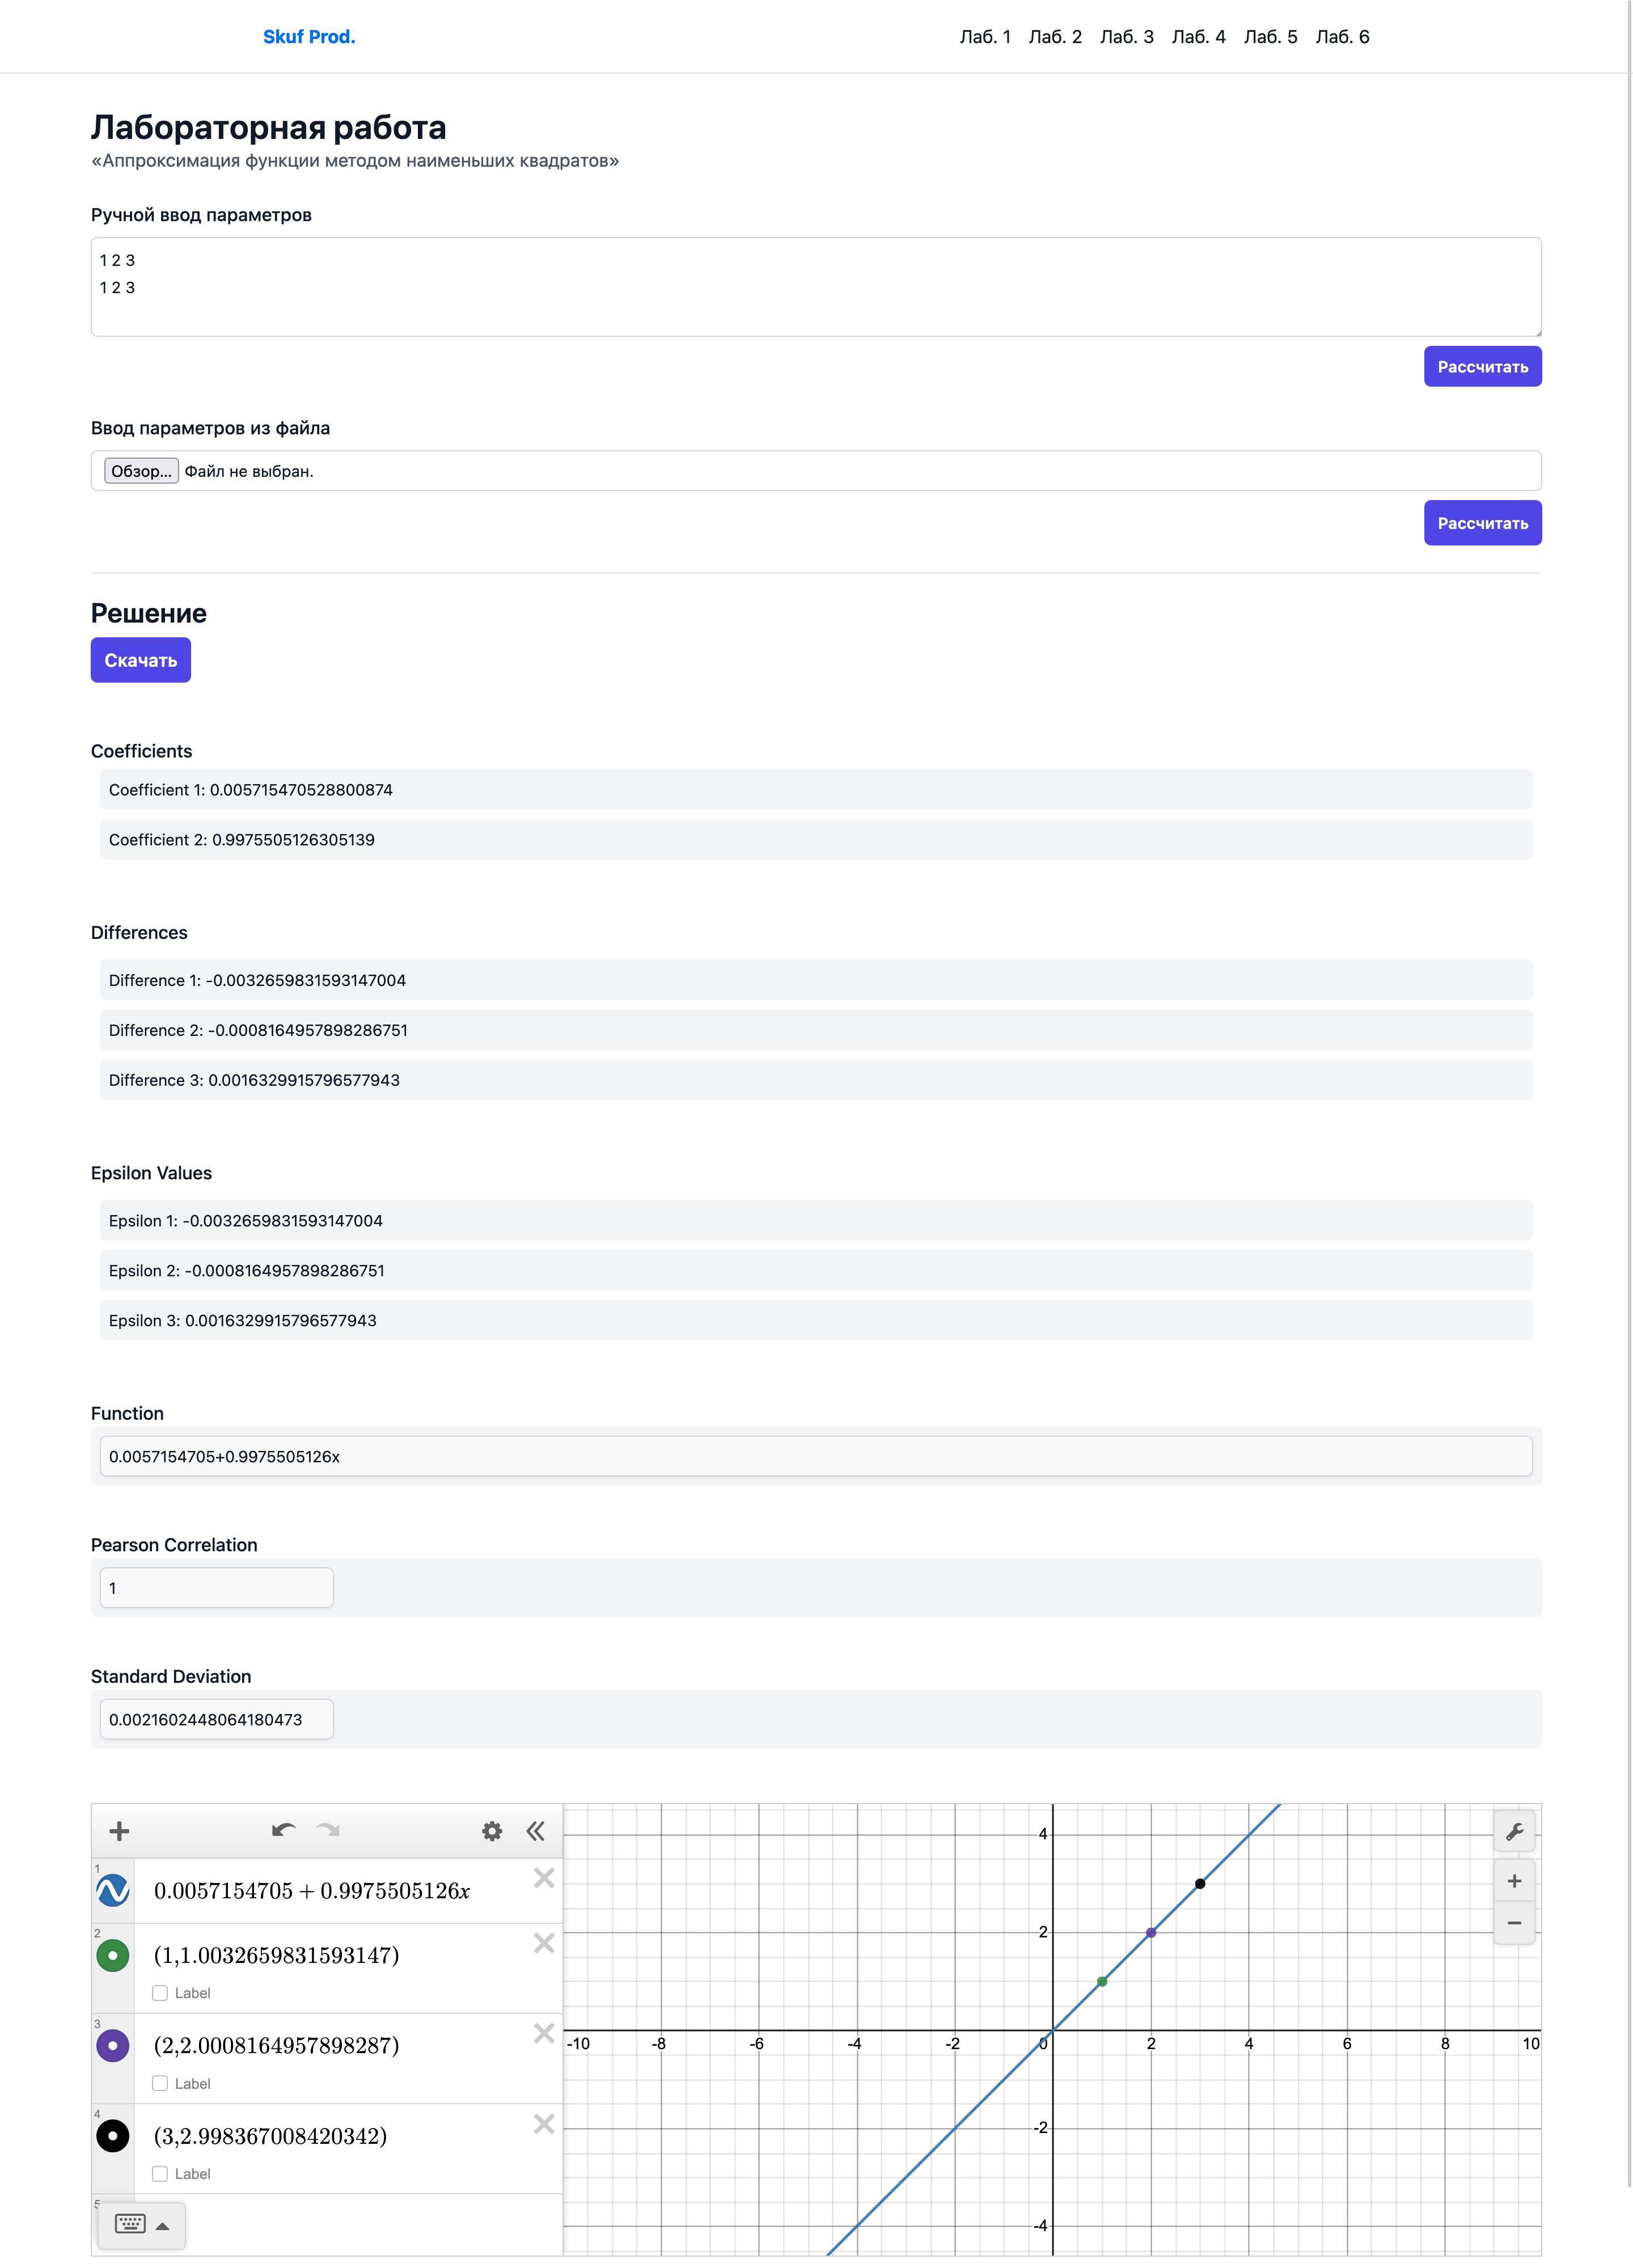
\includegraphics[scale=0.1]{ui.png}
                        \caption{\small \sl {UI  1}}  
                  \end{center}  
            \end{figure}
            
\section{Заключение}
      В ходе выполнения данной ЛР я ознакомился с основыми методами квадратичной аппроксимации. Вообще с кайфом написал программу и посчитал ручками.

\begin{thebibliography}{9}
    \bibitem{Методичка}Слайды с лекций (2023). // Кафедра информатики и вычислительной техники -- Малышева Татьяна Алексеевна, к.т.н., доцент.
\end{thebibliography} 

\end{document}
